%% Font size %%
\documentclass[11pt]{article}

%% Load the custom package
\usepackage{Mathdoc}

%% Numéro de séquence %% Titre de la séquence %%
\renewcommand{\centerhead}{Chap. 8 : Statistique à deux variables - Représentation}

%% Spacing commands %%
\renewcommand{\baselinestretch}{1} \setlength{\parindent}{0pt}

\begin{document}

\begin{multicols}{2}

\begin{exercice}[1][Nuage de points]
Représenter dans le repère le nuage de points associé à la série
statistique ci-dessous.

\begin{center}
\begin{tabular}{|c|c|c|c|c|c|}
\hline
$x_i$ & 0 & 2 & 5 & 7 & 5  \\
\hline
$y_i$ & 3 & 2 & 1 & 5 & 8 \\
\hline
\end{tabular}
\end{center}

\begin{center}
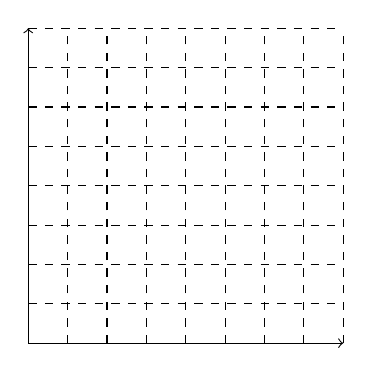
\begin{tikzpicture}[scale=0.5]
% Axes gradués
\draw[->] (0,0) -- (8,0); % Axe des x
\draw[->] (0,0) -- (0,8);  % Axe des y
% Grille en pointillés
\draw[dashed] (0,0) grid (8,8);
\end{tikzpicture}
\end{center}
\end{exercice}

\begin{exercice}[1][Nuage de points]
Représenter dans le repère le nuage de points associé à la série
statistique ci-dessous.

\begin{center}
\begin{tabular}{|c|c|c|c|c|c|}
\hline
$x_i$ & -3 & 0 & 3 & 5 & 8 \\
\hline
$y_i$ & 1 & -1 & -2 & 5 & 7 \\
\hline
\end{tabular}
\end{center}

\begin{center}
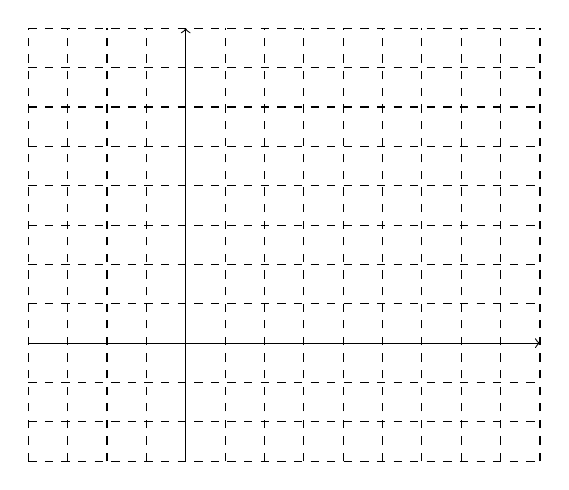
\begin{tikzpicture}[scale=0.5]
% Axes gradués
\draw[->] (-4,0) -- (9,0); % Axe des x
\draw[->] (0,-3) -- (0,8);  % Axe des y
% Grille en pointillés
\draw[dashed] (-4,-3) grid (9,8);
\end{tikzpicture}
\end{center}
\end{exercice}

\end{multicols}

\begin{exercice}[2][Point moyen]
\begin{multicols}{2}

Voici les valeurs prisent par une série statistique à deux variables.

\begin{center}
\begin{tabular}{|c|c|c|c|c|c|}
\hline
$x_i$ & 200 & 300 & 400 & 500 & 800 \\
\hline
$y_i$ & 3 & 5 & 7 & 10 & 12 \\
\hline
\end{tabular}
\end{center}

\begin{enumerate}
\item Représenter dans le repère le nuage de points associé à cette série
statistique ;
\item calculer la moyenne des $x_i$ ;
\item calculer la moyenne des $y_i$ ;
\item en déduire les coordonnées du point moyen et le placer dans le
repère ci-contre.
\end{enumerate}

\columnbreak

\begin{center}
\begin{tikzpicture}[scale=0.7]
% Axes gradués
\draw[->] (0,0) -- (9,0) node[right]{$x_i$}; % Axe des x
\draw[->] (0,0) -- (0,15) node[above]{$y_i$};   % Axe des y
% Graduations sur l'axe des x
\foreach \x in {0,1,...,9} {
    \draw (\x,0) -- (\x,-0.2) node[below]{ };
}
% Graduations sur l'axe des y
\foreach \y in {0,1,...,15} {
    \draw (0,\y) -- (-0.2,\y) node[left]{ };
}
% Grille en pointillés
\draw[dashed] (0,0) grid (9,15);
\end{tikzpicture}
\end{center}
\end{multicols}

\end{exercice}

\begin{multicols}{2}

\begin{exercice}[2][Point moyen]
Voici un tableau de valeurs représentant une série statistique à deux variables.

\begin{center}
\begin{tabular}{|c|c|c|c|c|c|}
\hline
$x_i$ & 23 & 56 & 78 & 34 & 89 \\ \hline
$y_i$ & 45 & 12 & 67 & 90 & 3 \\ \hline
\end{tabular}
\end{center}

\begin{enumerate}
\item calculer la moyenne des $x_i$ ;
\item calculer la moyenne de $y_i$ ;
\item en déduire les coordonnées du point moyen $G(\overline{x},\overline{y})$. 
\end{enumerate}
\end{exercice}

\begin{exercice}[3][Point moyen]
Voici un tableau de valeurs représentant une série statistique à deux variables.

\begin{center}
\begin{tabular}{|c|c|c|c|c|c|}
\hline
$x_i$ & -2 & 0 & 1 & 3 & 5 \\ \hline
$y_i$ & 1 & -1 & -2 & 5 & 10 \\ \hline
$u_i = \dfrac{1}{y_i}$ & \phm\phm & \phm\phm & \phm\phm & \phm\phm & \phm\phm \\ \hline
\end{tabular}
\end{center}

\begin{enumerate}
\item Compléter la troisième ligne du tableau en calculant les valeurs
des $u_i$ ;
\item calculer la moyenne des $x_i$ ;
\item calculer la moyenne de $u_i$ ;
\item en déduire les coordonnées du point moyen $G(\overline{x},\overline{u})$. 
\end{enumerate}

\end{exercice}

\end{multicols}

\begin{exercice}[4][Immatriculation des véhicules électriques]
Le tableau ci-dessous donne le nombre de véhicules électriques neufs
immatriculés en France de 2014 à 2018 (\textit{source :
  Avere-France}).

\begin{center}
\begin{tabular}{|c|c|c|}
\hline
Année & Rang de l'année \( x_i \) & Nombre de milliers de véhicules \( y_i \) \\
\hline
2014 & 0 & 10,5 \\
2015 & 1 & 17,3 \\
2016 & 2 & 21,7 \\
2017 & 3 & 24,9 \\
2018 & 4 & 31 \\
\hline
\end{tabular}
\end{center}

\medskip

\begin{multicols}{2}
\begin{enumerate}
\item Graduer correctement les axes du repère ci-contre ;
\item représenter la série statistiques sous forme d'un nuage de
points ;
\item en moyenne combien de voitures électriques on été immatriculées
entre l'année 2014 et 2018 ?
\item en déduire les coordonnées du point moyen puis placer ce point
dans le repère. \\ \\ \\ \\ 
\end{enumerate}


\begin{center}
\begin{tikzpicture}[scale=0.7]
% Axes gradués
\draw[->] (0,0) -- (10,0) node[right]{}; % Axe des x
\draw[->] (0,0) -- (0,10) node[above]{}; % Axe des y
% Graduations sur l'axe des x
\foreach \x in {0,1,...,10} { \draw (\x,0) -- (\x,-0.2) node[below]{
  }; }
% Graduations sur l'axe des y
\foreach \y in {0,1,...,10} { \draw (0,\y) -- (-0.2,\y) node[left]{ };
}
% Grille en pointillés
\draw[dashed] (0,0) grid (10,10);
\end{tikzpicture}
\end{center}
\end{multicols}
\end{exercice}


\end{document}

% Local Variables:
% gptel-model: deepseek-chat
% gptel--backend-name: "DeepSeek"
% gptel--bounds: ((356 . 484) (499 . 625) (637 . 1005) (1020 . 1148) (1160 . 1404) (1422 . 1456) (1476 . 1712) (1731 . 1732) (1738 . 1820) (1998 . 2493) (2508 . 2524) (2564 . 2663) (2677 . 2811) (3047 . 3146) (3160 . 3377) (3919 . 4154) (4564 . 5027))
% End:
